\documentclass[a4paper, 11pt, normalem]{report}

\usepackage{../../../LaTeX-Templates/Notes}

\title{Condensed Matter \\ Physics 3 \vspace{-20pt}}
\author{Dr Michael Hunt and Prof Tom Lancaster}
\date{\vspace{-15pt}Michaelmas Term 2018 - Epiphany Term 2019}
\rhead{\hyperlink{page.1}{Contents}}

\begin{document}
\maketitle
\tableofcontents

\part{Symmetry, Structure, and Excitations}
\chapter{}
\textbf{use alongside lecture notes given}

\textbf{Chapters in this don't always coincide to lectures - missed a few}

\begin{itemize}
    \item Solid:
        \begin{itemize}
            \item Can support sheer stress
            \item Doesn't flow
        \end{itemize}

    \item Liquid:
        \begin{itemize}
            \item Incompressible
            \item Can't support sheer stress
            \item Flows the fill volume, subject to remaining pressure
            \item Weaker forces ($\approx k_B T$)
            \item Less dense atoms/molecules
        \end{itemize}
\end{itemize}

A gas, liquid, or amorphous solid is rotationally invariant

N particles in a shell, what is $g(r)$?
\begin{equation}
    g(r) = \frac{N}{4\pi r^2\delta r\langle n\rangle}
\end{equation}

For an ideal gas (point particles), $g(r)$ is just 1:
\begin{itemize}
    \item $\int_V \langle n \rangle g(r)\,dV = (N' - 1)$
    \item $\langle n \rangle V g(r) = (N' - 1) \implies g(r) = 1 - \frac{1}{N'}$
    \item Despite rigidity of ice, it can be seen to flow.
    \item For enough stress, it will plastically deform (creep).
    \item "Enough" is about 5 orders of magnitude less than expected for a perfect crystal.
    \item Ice flows due to the motion of topological defects called dislocations. Electrons can scatter off them too.
    \item The pdf does not enable us to easily extinguish between a liquid and amorphous solid. The difference is one of timscale for flow.
    \item Therefore an arbitrary definition: "A solid is a material whose shear viscosity exceeds $10^{13.6} N\,s\,m^{-2}$"
    \item this corresponds to a relaxation time of about a day
\end{itemize}

\chapter{}

\section{Bonding in Condensed Matter}
In general, inter-particle interactions produce a potential with the same type of form, usual potential well plot with repulsive and attractive forces.
\textbf{image here from notes}

\subsection{van der Waals bonding}

Fluctuations (instantaneous in time) can lead to instantaneous dipole moments.
Such dipoles create an electric field:
\begin{equation}
    E = \frac{p_1}{4\pi\epsilon_0 r^3},
\end{equation}
where $p_1$ is the fluctuating dipole.
On a neighbouring atom, this field induces a dipole,
\begin{align}
    p_2 &= \alpha|E| \\
    p_2 &= \alpha \frac{p_1}{4\pi\epsilon_0 r^3}
\end{align}
where $\alpha$ is the atomic polarisability.
We have a dipole-dipole potential:
\begin{equation}
    U(r) = \frac{|p_1||p_2|}{4\pi\epsilon_0 r^3} = \frac{\alpha|p_1|^2}{(4\pi\epsilon_0)^2r^6}
\end{equation}
Note that $|p_1|^2$ does not average to zero even though p does, which implies that $U(r) \neq 0$.

If we have attractive interactions alone, our solid would collapse into a singularity.
We need repulsion as well.
Repulsion arises from the Pauli exclusion principle - no electrons (fermions) can have the same set of quantum numbers.
Born and Mayer parameterised this repulsion as
\begin{equation}
    U_{rep} = B_{ij}\exp{-\frac{r_{ij}}{p_{ij}}}
\end{equation}
where $r_{ij}$ is distance between atom i and j. $p_{ij}$ and $B_{ij_{}}$ are constants.

Buckingham potential - Historically, a potential varying as $r^{-n}$ is easier to deal with and reasonably reproduces $f^n$ form.
Lennard-Jones potential constants $\epsilon$ and $\sigma$ - parameters which can be found by experiment

\subsection{Ionic Bonding}

When it's energetically favourable to transfer one or more electrons to a neighbour to acheive a closed shell configuration.

$U_{\text{Madelung}_{}}$ is attractive interaction per mole of formular unit.

Born-Mayer is very short-ranged

\subsection{Metallic bonding}

Metallic bonding resutls from delocalisation of electrons.

The coulomb energy (attractive) can be found from a lattice sum (with negative charge background) and is $\propto \frac{1}{r}$.
Two results from FoP2B are required to understand the electronic contribution to energy.
The average energy electron is
\begin{align}
    \frac{E}{n} &= \frac{3}{5}E_F = \frac{3\hbar^2 k_{F}^2}{10m_e} \\
    k_F &= \left(3\pi^2\frac{N}{V}\right)^{1/3} \\
    k_F &\propto V^{-1/3} \\
    \implies \frac{E}{n} &\propto r_{0}^{-2} (\because V \propto r_{0}^{3}) \\
    U_{metal} &= U_{coul} + U_{kin} \\
    &= -\frac{a}{r_0} + \frac{b}{r_0^2}
\end{align}
Metallic crystal cohesive energy is of order of a few eV per atom.

\chapter{}

\textbf{check DUO for these}

\chapter{}

Thomson formula:
\begin{equation}
    \frac{d\sigma}{d\Omega} = r_e^2\frac{1 + \cos^2\theta}{2}
\end{equation}

Scattering amplitude
\begin{equation}
    \langle k'|V|k\rangle = \langle k'|r_e(r)|k\rangle
\end{equation}

\begin{itemize}
    \item Introduce $q = k' - k$, note vector relation, the scattering wavevector

    \item Fourier transforms used - atomic scattering factor (scattering potential of each atom, summed over all)

    \item $I(q)$ depends on structure, $|f_a|^2$ depends on atoms

    \item $\frac{I(q)}{N} = S(q)$ - the target structure factor
\end{itemize}

\section{Xray scattering and pair distribution}

\begin{itemize}
    \item Assume homogeneous material, translationally variant
    \item There is a '-1' due to avoidance of counting "oneself" - reference atom
    \item $\langle n(x_i)\rangle = \langle n(x_2)\rangle = n$
\end{itemize}

\section{Xray scattering in periodic lattice}

The expression
\begin{equation}
    I(q) = \sum_{j,l} \langle e^{iq \cdot R_{jl}}
\end{equation}
$R_{jl} = R_j - R_l$.
Summing over all atoms yields $N^2$ terms.
If $R_j - R_i$ is random, this sums to 0 as $N \to \infty$.
Therefore, for non-zero $I(q)$, we must have $q\dot R_{jl} = 2m\pi_{}$ where m integer.

We can express the lattice points in terms of three basis vectors.
\begin{equation}
    R_{jl} = U\vec{a} + V\vec{b} + W\vec{c}
\end{equation}
Since $R_j - R_l$ must be a lattice vector.

For non-zero $I(q)$, let's define a set of vectors $\vec{a}^{*}, \vec{b}^{*}, \vec{c}^{*}$.*

Atoms in the unit cell for the convolution

Written Fourier transform of lattice.
For electrons in an atom, we have shown above that F.T. is atomic scattering amplitude, $f_j$.
An atom at position $r_j$ in a unit cell can be represented as delta fn, which has F.T. exp.
For more than one atom in unit cell, can sum over them so last two terms in F(structure) become
\begin{equation}
    \sum_j f_j e^{iq\dot r_j}
\end{equation}
We can write position of atoms within the unit cell in fractional coordinates.

Lattice is only non-zero when $q = G_{hkl_{}}$.
We can therefore write the lattice structure factor

\begin{equation}
    F(hkl) = \sum_j f_j(q)e^{2\pi i(hx + ky + lz)}
\end{equation}

\chapter{}

\begin{align}
    \vec{k}\cdot\vec{G} &= \sin\theta = -\vec{k}'\cdot\vec{G} \\
    G &= \frac{2\pi}{\lambda}\Delta k \\
    |G| &= \frac{2\pi}{\lambda}(2\sin\theta) \\
    \lambda &= 2\left(\frac{2\pi}{|G|}\right)\sin\theta \\
    &= 2d\sin\theta
\end{align}

\chapter{}

\begin{itemize}
    \item Neutron scattering factors can allow access to information complementary to xray scattering
        (very little angular dependence in $b_i$ due to small size of nucleus)
    \item Point symmetry operations are those carried about a point, they do not involve translation
    \item The identity operation is given the symbol 1 in "International Notation". [However, in Schoenflies Notation, it has the symbol E.]
    \item An n-fold rotation axis exists if a rotation of $360/n$ brings an object back into coincidence with itself.
    \item \textit{see notes for images of rotation axes}
    \item \textit{see notes for various rotation stuff}
    \item Rotoinversion axes consist of two steps:
        \begin{enumerate}
            \item Rotation, followed by
            \item Inversion
        \end{enumerate}
        \vspace{8pt}
        An n-fold rotoinversion axis is given the symbol $\bar{n}$.
        The simplest rotoinversion axis is $\bar{1}$ - the centre of inversion symmetry.
    \item In practice, we find that we need to combine symmetry operations.
        Consider a mirror plane which is perpendicular to a 2-fold rotation axis.
    \item Combinations can generate other symmetry operations.
    \item Note that you don't need commutativity - AB not necessarily equal to BA
\end{itemize}

\chapter{}

\section{Lattices and Symmetry}
Recall from section 2.1.5, Lecture 4, we can define translation vectors $\vec{a},\vec{b},\vec{c}$ and that these enable us to mathematically define a lattice.
\begin{equation}
    \La(\vr) = \sum_{u,v,m} \delta(\vr - (U\vec{a} + V\vec{b} + W\vec{c}))
\end{equation}
We can use these vectors to define a parallelepiped with sides a, b, c (moduli of vectors) and angles $\alpha, \beta, \gamma$.

Symmetry imposes constraints on our choice of basis, or lattice, vectors $\vec{a},\vec{b},\vec{c}$.
In the above case the 4-axis (conventionally along c) means that $a=b$ and $\alpha=\beta=\gamma=\SI{90}{\degree}$.

For a lattice with mirror plane:\\
One axis must be perpendicular to mirror plane (let's define as $\vec{c}$).
Other two aces must be in the plane of the mirror.
This constrains us to $\alpha=\beta=\SI{90}{\degree}$.

Once we build a 3D crystal by stacking planes something something something he moved the slides away

\section{The 14 Bravais Lattices}
It's often usful to consider non-primitive unit cells (cells with more than one lattice point) so that we can group structures of similar defining symmetry.
The complete set of lattices which can be derived from our 7 crystal systems are the 14 Bravais lattices.

These lattices are labelled as followed:
\begin{itemize}
    \item P - primitive
    \item I - body-centred
    \item F - face-centred (for all faces)
    \item R - rhombohedral
    \item A,B,C - face-centred (on one face A, B, or C only)
\end{itemize}
A crystal structure is generated by placing a group of atoms or molecules - a motif (or basis) - at each lattice point.
This is a convolution.
\begin{equation}
    \La(\vr) \ast \text{motif}
\end{equation}
Motif being the positions given by fractional co-ordinates within cell.

\section{Translation Symmetry and Space Groups}

A screw axis involves a $\frac{\SI{360}{\degree}}{n}$ rotation followed by translation along the axis by a fraction of a lattice vector, $\frac{1}{t}$.
This is labelled
\begin{equation}
    n_m,~ m = \frac{n}{t}, n = \text{rotation axis}
\end{equation}

Screw axis shown is a $2_1$ axis.

We can have a,b,c glide planes where the label indicates the direction of translation.
We can also define an n-glide which involves translation along $\frac{1}{2}(\vec{a}+\vec{b})$ and a d-glide (diamond glide) which involes translation along the diagonal of the unit cell.

We label the space group of a crystal by combining the symbol for the conventional lattice with the symbols for the symmetry operations, e.g. the face-centred cubic structure with full symmetry would be:
\begin{equation}
    Fm\bar{3}m
\end{equation}
Consider a rhombohedral crystal, with: an n-glide plane along (100); a mirror with reflection in (010); and an a glide with reflection in (001).
This would have space group
\begin{equation}
    Pnma.
\end{equation}

\section{Symmetry and Diffraction}
Recall our expression for the lattice structure factor (Lecture 4, Section 2.1.5)
\begin{equation}
    F(hkl) = \sum_{\text{unit cell}} f_j(\vec{q}_{hkl})e^{2\pi i(hx_j + ky_j + lz_j)}
\end{equation}
By inspection, for real $f_j$, $F(\bar{h},\bar{k},\bar{l}) = F^*(hkl)$.
In a scattering experiment, we detect $|F|^2$, and $|F(hkl)|^2 = |F(\bar{h}\bar{k}\bar{k})|^2$, i.e. all diffraction patterns (where there's no anomalous scattering) have a centre of symmetry.
This means that the point group symmetry measured - the Laue symmetry is the real symmetry plus a centre of inversion.

\textbf{Note: several further lectures after this that I didn't attend, check duo}

%%%%%%%% BROKEN SYMMETRY HERE, SORT OUT FILES

\part{Broken Symmetry}
\chapter{Introduction to Broken Symmetry}
\begin{itemize}
    \item Standard Tom Lancaster style - take note of what he does on visualiser, also check slides but not as important
\end{itemize}

\section{Phase diagram of water}
\begin{enumerate}
    \item Solid to liquid - symmetry is changed
    \item liquid to gas - no change in symmetry (can avoid discontinuity)
\end{enumerate}
\begin{itemize}
    \item Distinguish two types of transition - no critical end point on melting curve
    \item For many phenomena, symmetry is broken (lowered) at a critical temperature, $T_c$
\end{itemize}
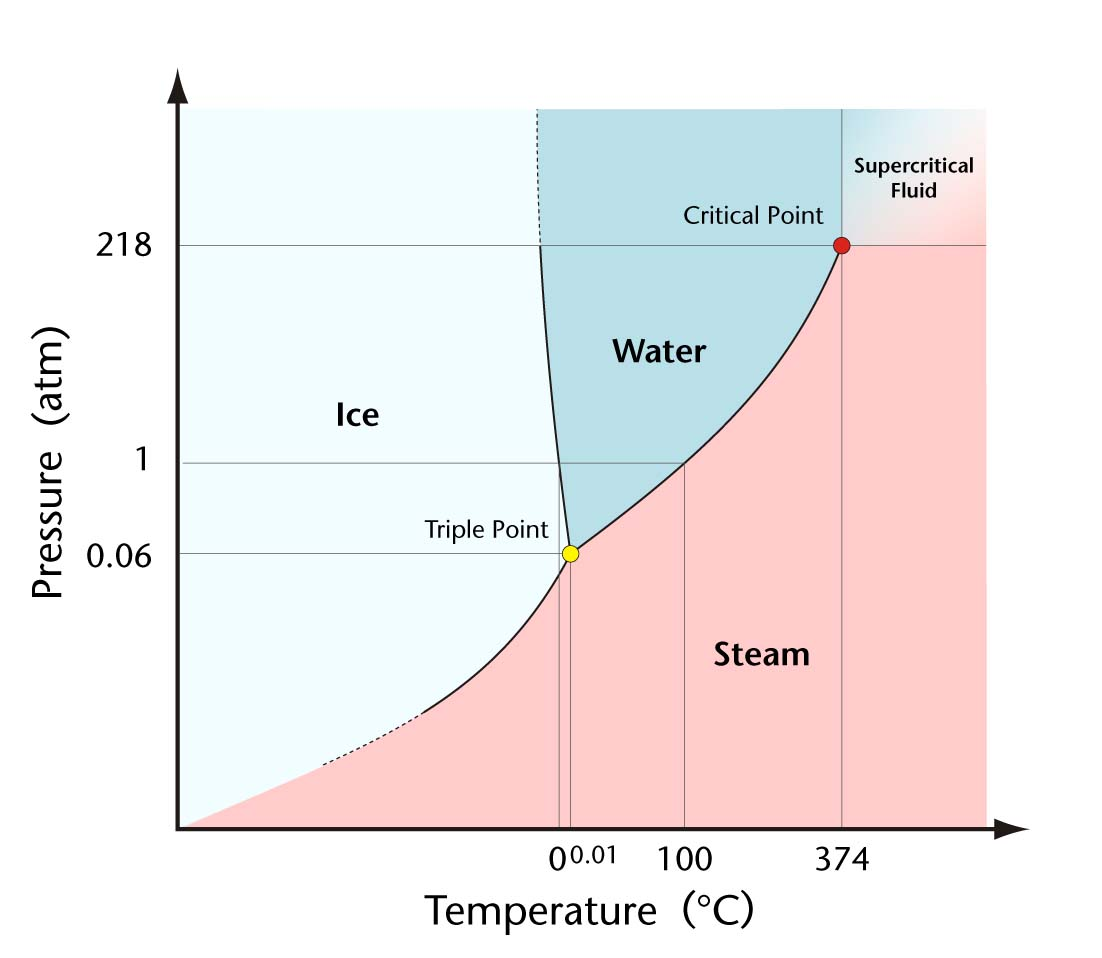
\includegraphics[scale=0.5]{water.png}
Make this side on

\section{Landau Theory of Phase Transitions}
Free energy: 
\begin{align}
    F &= U - TS \\
    M &= \text{magnetization}\frac{\text{magnetic moment}}{\text{volume}} \\
    F &= F_0 + aM^2 + bM^4 + \cdots
\end{align}
With no odd powers, this has a symmetry
\begin{align}
    M &\to -M \\
    F(M) &= F(-M)
\end{align}
This is a symmetry - a $Z_{\lambda}$ symmetry

Plot a graph of it in either a rough parabola or cubic function centred on 0, depending on whether $a,b,M >,<,= 0$.
\begin{align}
    \frac{\p F}{\p M} &= 2aM + 4bM^3 = 0 \\
    \text{Minima at } M &= 0 \\
    \text{Minima at } M^2 &= \frac{-a}{2b}
\end{align}
Take $a = a_0(T-T_c)$, changes sign at $T_c$:
\begin{align}
    a_{+ve} &\to T>T_c \\
    a_{-ve} &\to T<T_c \\
    M &= \pm \left[\frac{a_0}{2b}(T_c-T)\right]^{1/2}
\end{align}
Model has predicted a phase transition at $T_c$.

\begin{itemize}
    \item We define the 'order parameter':
        \begin{equation}
            \text{Order parameter} = \begin{cases} 0 & T > T_c \\ \cancel{0} & T < T_c \end{cases}
        \end{equation}
        (Magnetization for a magnet)
    \item Impossible to change symmetry gradually - phase transitions are too sharp
    \item System can break symmetry in $> 1$ way(s).
    \item Consequences of broken symmetry:
        \begin{itemize}
            \item Phase transitions
            \item Rigidity
            \item Excitations
            \item Defects
        \end{itemize}
\end{itemize}

\chapter{}

\chapter{}
\section{Models and Dimensionality}
\begin{itemize}
    \item Model a system as spins on a lattice
    \item Hamiltonian, 
        \begin{equation}
            H = \sum_{\langle ij\rangle} \left(-J_{ij}\right) \vec{S}_i\cdot\vec{S}_j
        \end{equation}
    \item $J > 0$: ferromagnetism is most likely
    \item D - dimensionality of the spin
    \item $D=1$, $S_z = \pm 1$ - known as Ising models
    \item $D=2$, $S_x,S_y$ - XY model
    \item $D=3$, $S_x,S_y,S_z$ - Heisenberg model
    \item d - dimension of the lattice
    \item \textbf{Example: } $d=1,D=1$ (1d Ising model) \\
        N spins, up - each one has $-J/4$, if $S = 1/2$ - $F_0= -(N-1)J/4$, entropy $S=0$
    \item Put in mistake, of down state too - Energy cost $J/2$, entropy gain $k_B\ln(N-1)$, $N-1$ places to put the wall
        \begin{equation}
            F_1 = -(N-1)\frac{J}{4} + \frac{J}{2} - k_BT\ln(N-1)
        \end{equation}
        Now let $N \to \infty$: energy cost is constant, entropy gain $\to \infty$.
        $F_1 < F_0$ when $k_BT\ln(N-1) > \frac{J}{2}$. \\
        So we conclude, No LRO for $T > 0$, no phase transition $\to$ no ferromagnetism
    \item General result, $d=1$ systems don't show a phase transition. 
    \item 2d Ising model ($D=1,d=2$) - Can be solved, there is a phase transition. (Onsager, 1940s)
\end{itemize}

\section{Critical Exponents}
Most things in Physics depend on scale, e.g. $e^{-t/\tau},~e^{-x/L}$. It's remarkable when they don't, e.g. $t^\delta$ - a power law. 

\begin{example}[Phase transitions]
    \begin{align}
        M &= \alpha(T_c-T)^\beta
    \end{align}
    In general, $\beta$ will depend on $d,D$.
    Consider the Landau theory from Lecture 1, $\beta = \frac{1}{2}$ in mean field theory.
\end{example}

\subsection{Other critical exponents}
\begin{itemize}
    \item Consider magnet in an applied field, $H$,
        \begin{align}
            F &= F(M) - \mu_0MH \\
            M &\propto (T_c-T)^\beta,~ T < T_c,~ H=0
        \end{align}
    \item Specific heat, 
        \begin{align} 
            C &\propto |T_c-T|^{-\alpha},~ T\to T_c,~ H=0
        \end{align}
    \item Susceptibility,
        \begin{align}
            \frac{M}{H}\bigg|_{H\to 0} = \chi &\propto |T-T_c|^{-\gamma}, T\to T_c,~ H=0
        \end{align}
    \item 
        \begin{equation}
            M \propto H^{1/\delta}, T = T_c
        \end{equation}
    \item Coherence length, 
        \begin{equation}
            \zeta \propto |T-T_c|^{-\nu}, H=0
        \end{equation}
    \item These are often written in terms of 'reduced T':
        \begin{equation}
            T = \frac{T-T_c}{T_c}
        \end{equation}
    \item Universality is the notion that critical exponents depend on d, D, and whether interactions are long or short range
\end{itemize}

\section{Scaling Relations}
Consider 4 exponents, $\alpha, \beta, \gamma, \nu$ - only 2 are independent.
\begin{itemize}
    \item Widom hypothesis
        \begin{equation}
            \alpha + 2\beta + \gamma = 2
        \end{equation}
    \item Kadanoff relation
        \begin{equation}
            \alpha = 2 - \nu d
        \end{equation}
\end{itemize}

\chapter{}

Sort another lecture

\chapter{Excitations}
\section{Spin waves in a magnet}
\begin{itemize}
    \item Two "modes" in "wine bottle"
        \begin{enumerate}
            \item Goldstone mode - rolling in the gutter
            \item Climbing the walls
        \end{enumerate}
    \item Goldstone's theorem - \emph{whenever you break a continuous global symmetry, it's possible to make an excitation for vanishingly small energy costs}
\end{itemize}
For a $D=3$ model:
\begin{align}
    H &= -\sum_{\langle ij\rangle} J\unl{S}_i\cdot\unl{S}_j = -J\sum_i \unl{\hat{S}}_i\cdot\unl{\hat{S}}_{i+1} \\
      &= -J\sum_i S_i^z S_{i+1}^z + \frac{1}{2} \left(S_i^+S_{i+1}^- + S_i^-S_{i+1}^+\right)
\end{align}

\begin{itemize}
    \item Rules:
        \begin{align}
            S^z|\uparrow\rangle &= \frac{1}{2}|\uparrow\rangle & S^z|\downarrow\rangle &= -\frac{1}{2}|\downarrow\rangle \\
            S^+|\uparrow\rangle &= 0 & S^+|\downarrow\rangle &= |\uparrow\rangle \\
            S^-|\uparrow\rangle &= |\downarrow\rangle & S^-|\downarrow\rangle &= 0
        \end{align}
    \item Ground state
        \begin{equation}
            |\Phi\rangle = |\uparrow\uparrow\uparrow\uparrow\uparrow\rangle,~ E = -\frac{NJ}{4}
        \end{equation}
    \item Flip a spin:
        \begin{align}
            |j\rangle &= |\uparrow\uparrow\uparrow\uparrow\uparrow\downarrow\uparrow\uparrow\uparrow\rangle = S_j^-|\Phi\rangle \\
            H|j\rangle &= \left(-\frac{NJ}{4} + J\right)|j\rangle \\
                       &= -\frac{J}{2}|j+1\rangle  - \frac{J}{2}|j-1\rangle
        \end{align}
    \item Conclusion: $|j\rangle$ is not an eigenstate of $H$.
    \item Try a different ansatz: spin wave
        \begin{equation}
            |q\rangle = \frac{1}{\sqrt{N}} \sum_j e^{iqja}|j\rangle
        \end{equation}
        \begin{itemize}
            \item a - lattice spacing
            \item q - wave vector
            \item j - number
            \item 1 spin flip, shared between N spins
        \end{itemize}
        \begin{align}
            H|q\rangle &= \frac{1}{\sqrt{N}} \sum_j e^{iqja}H|j\rangle \\
                       &= \left(-\frac{NJ}{4} + J - \frac{J}{2}e^{iqa} -\frac{J}{2}e^{-iqa}\right)|q\rangle \\
                       &= \left[-\frac{NJ}{4} + J(1-\cos(qa))\right]|q\rangle
        \end{align}
        Therefore $|q\rangle$ is an eigenstate.

        \begin{figure}[H]
            \centering
            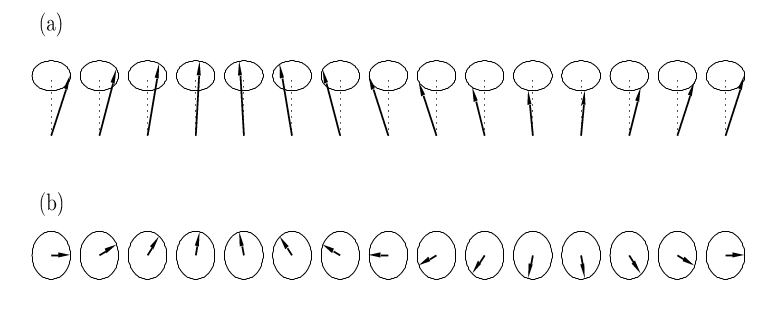
\includegraphics[scale=0.5]{spinrot.png}
        \end{figure}
\end{itemize}

\section{Energy above the ground state}
\begin{align}
    \hbar\om(q) &= J(1-\cos(qa))
\end{align}
\begin{itemize}
    \item \emph{Plot graph here}
    \item $\om \approx q^2$ for small $q$
    \item Spin waves are quantised into magnons
        \begin{itemize}
            \item At low T, only small $\om,q$ are important
            \item The number of states in general in 3D is 
                \begin{equation}
                    N(q) \approx q^3
                \end{equation}
            \item Density of states:
                \begin{align}
                    g(q)\,dq \approx q^2\,dq
                \end{align}
            \item For magnons, 
                \begin{equation}
                    g(\om)\,d\om \approx \om^{1/2}\,d\om
                \end{equation}
        \end{itemize}
\end{itemize}

\section{Remarks}

\begin{itemize}
    \item $S=1$ spin (1 spin flipped)
    \item Bosons
    \item "massless" - $\om \to 0, q \to 0$
    \item "Goldstone modes"
    \item Goldstone's theorem - \emph{whenever a continuous symmetry is broken, we get a new massless excitation}
    \item Conclusions:
        \begin{itemize}
            \item Breaking a continuous symmetry gives rise to a new mode of excitation
            \item These "Goldstone modes" can be excited for vanishing energy cost
            \item Magnons are the Goldstone bosons of the ferromagnet
            \item Some cases will not have these bosons due to Higgs mechanism
        \end{itemize}
\end{itemize}

\chapter{\textit{Lecture 9}}
\begin{itemize}
    \item Consider standard cubic about zero, wells for v and -v
    \item Broken symmetry potential
        \begin{align}
            f &= \frac12(\del\phi)^2 U(\phi) \\
            U(\phi) &= \frac{\lambda}{4}(v^2 - \phi^2)^2 \\
            v^2 &= \frac{u^2}{\lambda}
        \end{align}
    \item Most systems break symmetry in the same way, i.e. whole system will sit at v
    \item Alternatively if sitting in both wells, field plots between the two - called a wall, kink, or soliton
    \item Suppose a kink is of size l (in 1D) - Energy cost:
        \begin{align}
            \int \frac12 \left(\frac{\p\phi}{\p x}\right)^2dx &\approx l\left(\frac{v}{l}\right)^2 \\
                                                                &\approx \frac{v^2}{l}
        \end{align}
    \item To reduce the cost, we smear out the wall
    \item However, there's a second term
        \begin{align}
            \int U\,dx &= \lambda v^4l \\
            E &= \frac{v^2}{l} + \lambda v^4l \\
            \frac{\p E}{\p l} &= -\frac{v^2}{l^2} + \lambda v^4 = 0 \\
            l &= \left(\frac{1}{\lambda v^2}\right)^{1/2} \approx \frac{1}{\mu}
        \end{align}
    \item $E(x)$ forms like a Gaussian, kink is localised in a region of size l
    \item Center can be anywhere
    \item It costs a (semi-)infinite energy to remove it
        \begin{itemize}
            \item it's stable
        \end{itemize}
\begin{figure}[H]
    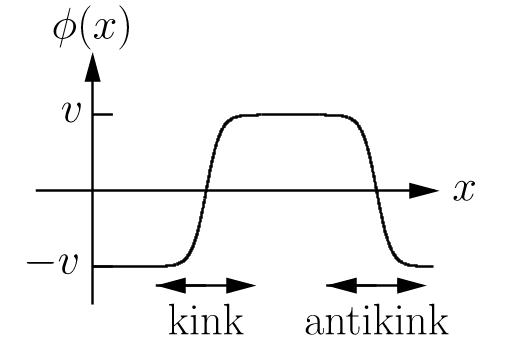
\includegraphics[scale=0.5,center]{kink.png}
\end{figure}
    \item Can unwind for only a finite energy cost
    \item What about vortices?
    \item Swirly at $r\to\infty$
    \item Costs a huge amount of energy
    \item Derrick's theorem: \emph{Time-independent topological objects are impossible to realise in greater than one spatial dimension for this theory}
    \item Contradictions to this:
        \begin{itemize}
            \item time dependence
            \item vortex-antivortex pairs
            \item add a field that cancels the effects of the swirliness
        \end{itemize}
\end{itemize}












\end{document}
